%# -*- coding: utf-8-unix -*-
%%==================================================

\chapter{树和二叉树}
\label{chap2}

\begin{itemize}[noitemsep,topsep=0pt,parsep=0pt,partopsep=0pt]
	\item 知识点:讲解相关知识点。
	\item 题型:直接上真题。
\end{itemize}

\section{知识点和方法论}

\subsection{知识点}
\begin{itemize}[noitemsep,topsep=0pt,parsep=0pt,partopsep=0pt]
	\item 树和森林的遍历与二叉树遍历的对应关系
	~\\
	\begin{center}
	\begin{tabular}{|c|c|c|}% 通过添加 | 来表示是否需要绘制竖线
		\hline  % 在表格最上方绘制横线
		先根遍历 & 先序遍历 & 先序遍历 \\
		\hline  %在第一行和第二行之间绘制横线
		后根遍历 & 中序遍历 & 中序遍历 \\
		\hline % 在表格最下方绘制横线
	\end{tabular}
	\end{center}
	\item 树的高度(深度)是从1开始计算的
	\item 公式$总结点数 = 总分支数 + 1   ==>  N2 + N1 + N0 = N1 + 2*N2 + 1$
	\item 完全二叉树的公式(二叉树的节点序号从1开始) $ 当 i \le \lfloor n/2 \rfloor $ 则节点i为分支节点,否则为叶子节点。
	\item 层次遍历二叉树,BFS,DFS的应用。
	\item 并查集的应用 参考链接 \url{https://blog.csdn.net/liuyang981122/article/details/81530014} 杭电复试笔试 \url{https://blog.csdn.net/weixin_42044546/article/details/88876958}
	\item 树的结点个数 = 树的边数+1
\end{itemize}
\begin{lstlisting}[basicstyle=\small\ttfamily, caption={}, numbers=none]
Staus InOrderTrav(BiTree T,Status(* Visit)(TElemType e)){
	//中序遍历二叉树T的非递归算法,对每个数据元素调用函数visit.
	InitStack(S);  Push(S,T);    //根指针进栈
	while(!StackEmpty(S)){
		while((GetTop(S,p)&&p)  Push(S,p->lchild);//p赋值转换,向左走到尽头
		Pop(S,p);  //空指针退栈
		if(!StackEmpty(S)){   //访问结点,向右一步
			Pop(S,p); if(!Visit(p->data)) return error;
			Push(S,p->rchild);
		} //if
	} //while
	Return ok;
} //InOrderTraverse
\end{lstlisting}

\subsection{方法论}
\begin{enumerate}[noitemsep,topsep=0pt,parsep=0pt,partopsep=0pt]
\item 把树和森林转化为二叉树处理
\item 对应看
\item 画出森林
\begin{itemize}[noitemsep,topsep=0pt,parsep=0pt,partopsep=0pt]
\item 首先画出二叉树
\item 把二叉树的右子树断开,变为树
\item 把右子树移动一定的角度 然后再断开兄弟节点,然后连接双亲节点
\end{itemize}
	 首先画出二叉树
	 把二叉树的右子树断开,变为树
	 把右子树移动一定的角度 然后再断开兄弟节点,然后连接双亲节点
\item 表示方法
\begin{itemize}[noitemsep,topsep=0pt,parsep=0pt,partopsep=0pt]
	\item 孩子兄弟表示法
	\item 孩子表示法像邻接表那样的
\end{itemize}

\item 森林表示为二叉树
\begin{itemize}[noitemsep,topsep=0pt,parsep=0pt,partopsep=0pt]
	\item 先把兄弟链断开
	\item 依次作为右子树的节点
\end{itemize}

\item 二叉树的中序线索化
\begin{itemize}[noitemsep,topsep=0pt,parsep=0pt,partopsep=0pt]
	\item 写出中序的序列然后根据中序的序列画上图片,哪一个是先,哪一个是后一目了然
\end{itemize}

\end{enumerate}


\section{真题实战}


\subsection{2017年第1题}


\begin{lstlisting}[basicstyle=\small\ttfamily, caption={}, numbers=none]
已知二叉树的现需,中序,后续遍历的结果分别如下,请 
1) 画出这个二叉树
2) 补齐遍历中的空白处
3) 画出中序线索化二叉树形。
先序序列 : _B_F_ICEH_G
中序序列 : D_KFIA_EJCG
后序序列 : DKIF_HJEGCA
\end{lstlisting}

解:
\begin{lstlisting}[basicstyle=\small\ttfamily, caption={}, numbers=none]
易知
DLR ABDFKICEHJG
LDR DBKFIAHEJCG
LRD DKIFBHJEGCA
\end{lstlisting}

\begin{figure}[H]
	\centering  % 环境中的内容居中排版
	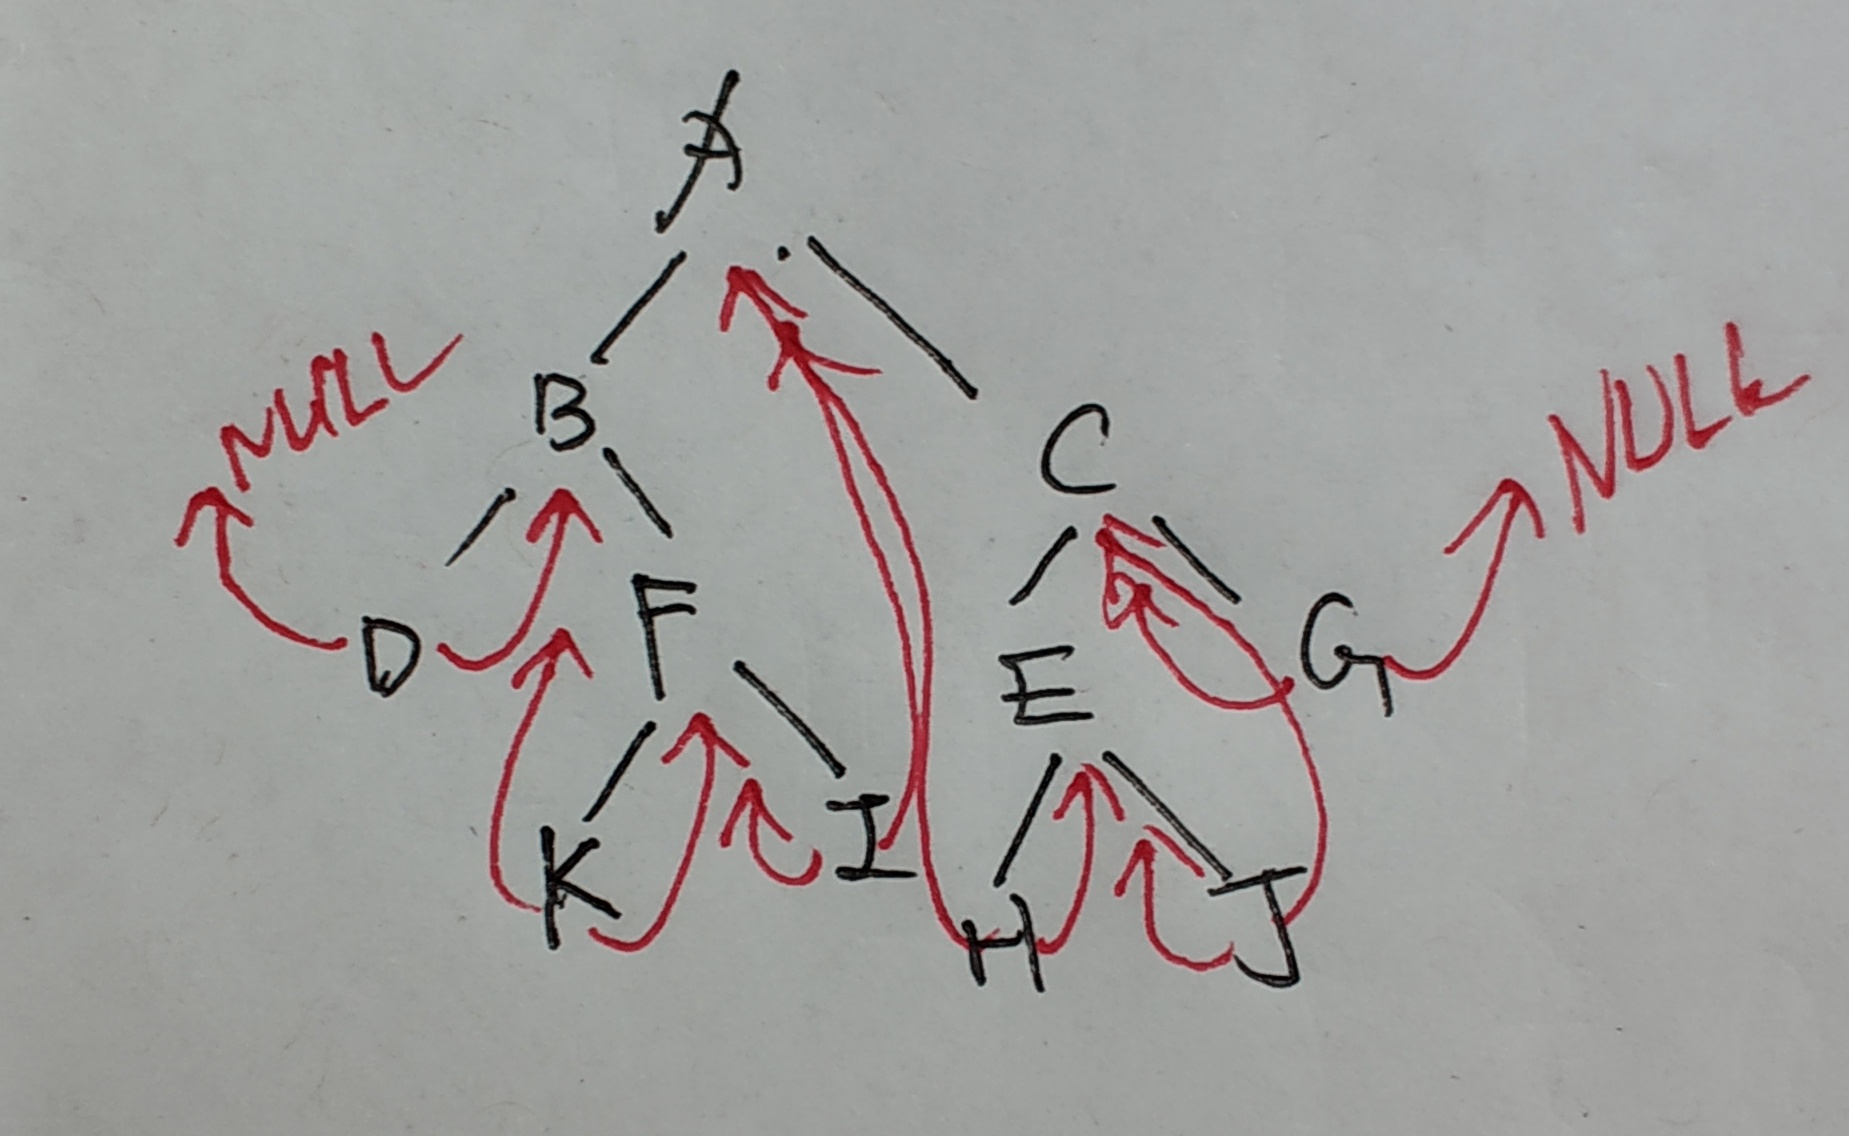
\includegraphics[scale=0.3]{example/chapter2/bitree20171.png}
\end{figure}


\subsection{2014年第3题}


\begin{figure}[H]
	\centering  % 环境中的内容居中排版
	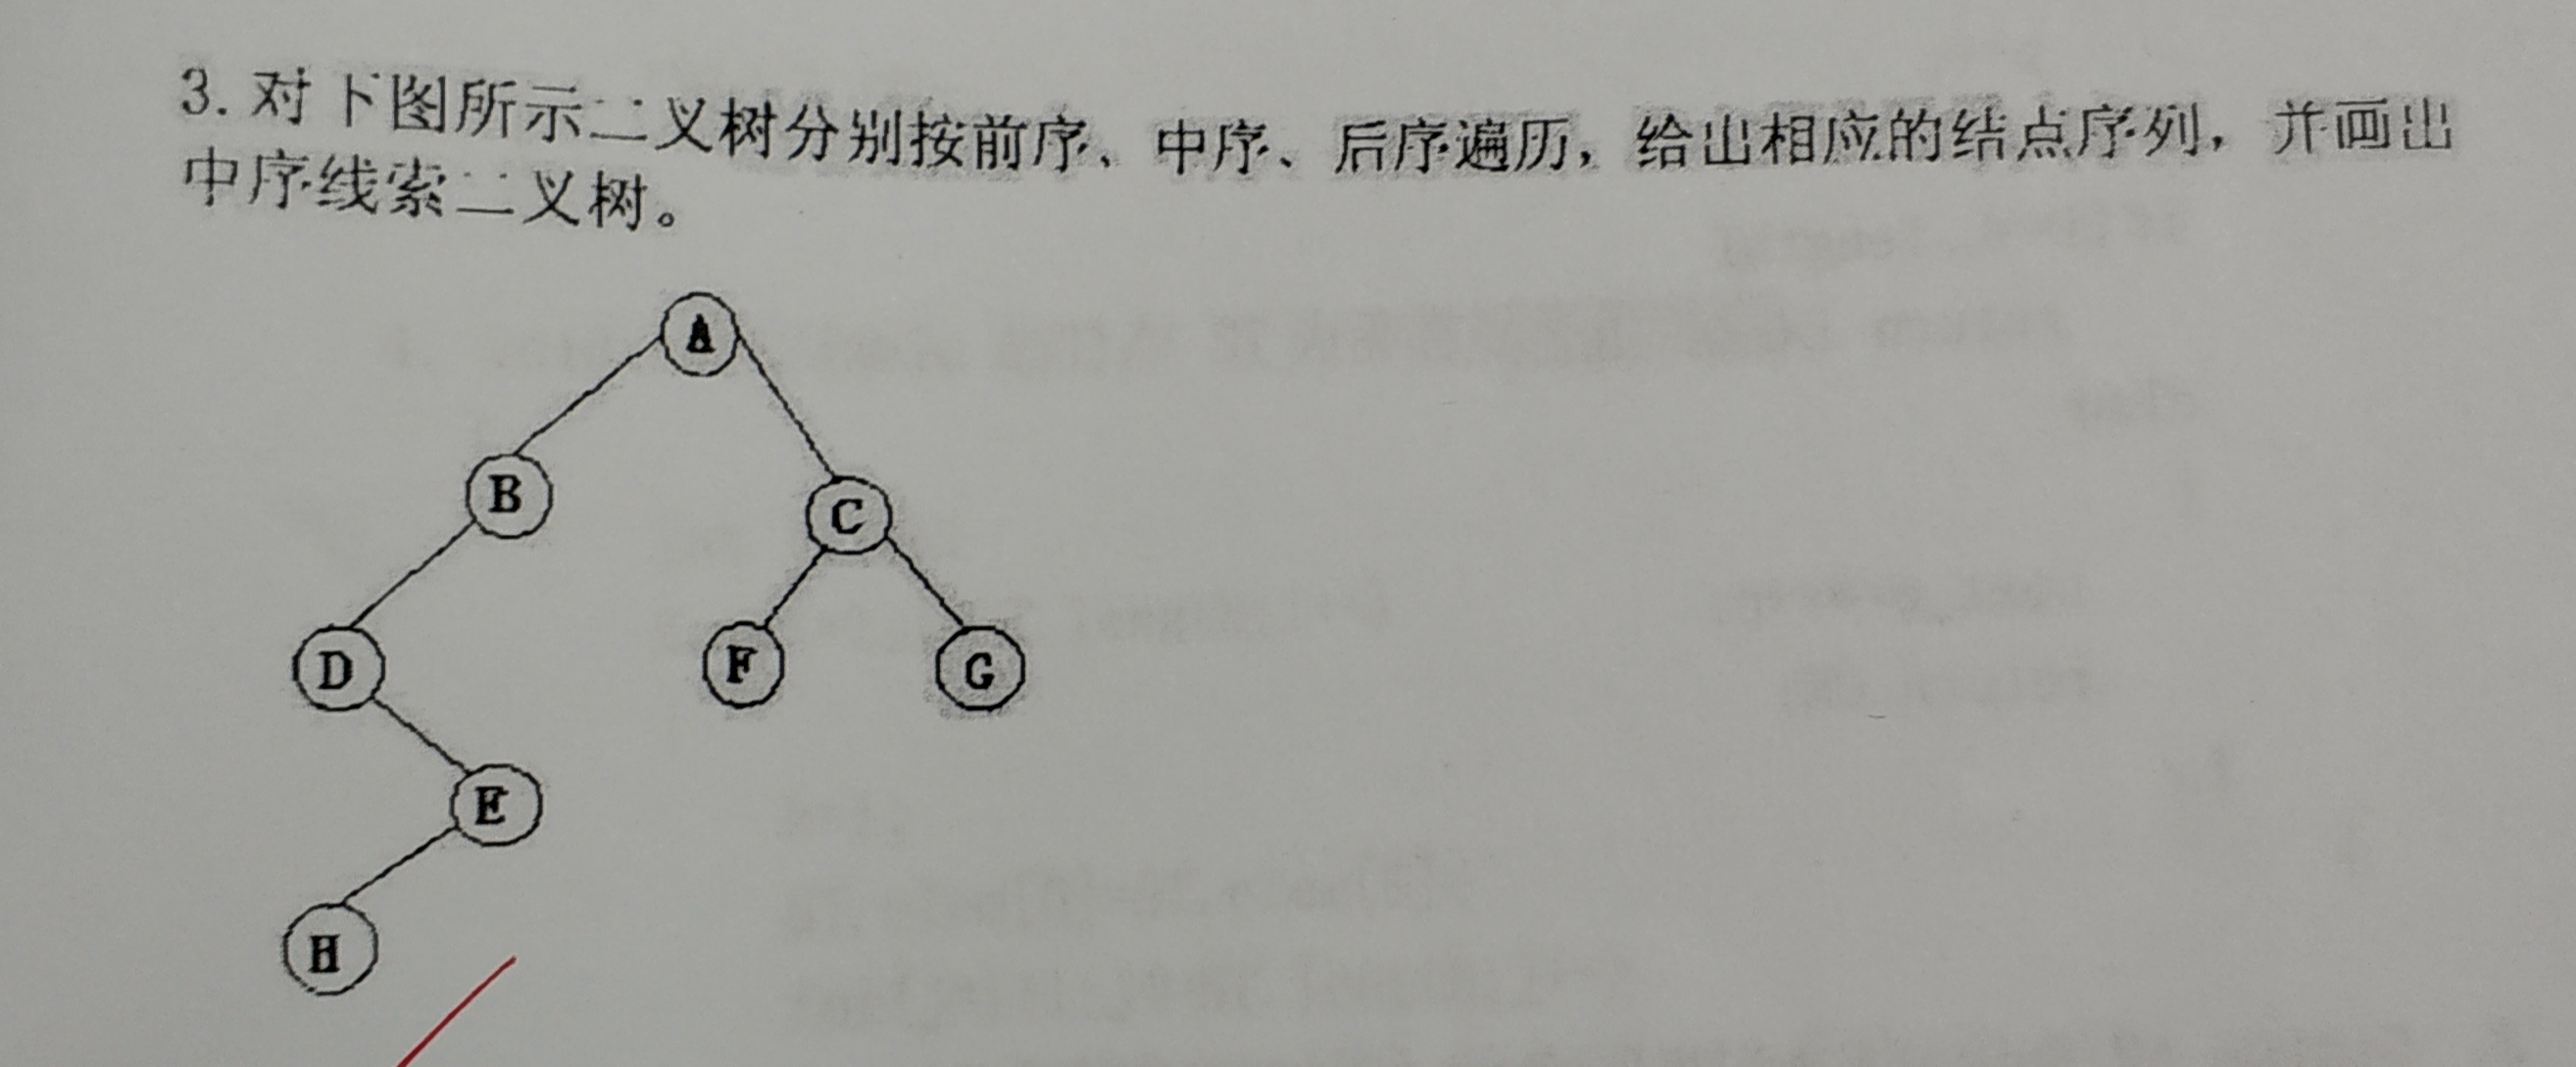
\includegraphics[scale=0.3]{example/chapter2/bitree20143.png}
\end{figure}

解:

\begin{lstlisting}[basicstyle=\small\ttfamily, caption={}, numbers=none]
易知
DLR  A B D E H C F G
LDR  D H E B A F C G
LRD  H E D B F G C A
\end{lstlisting}

\begin{figure}[H]
	\centering  % 环境中的内容居中排版
	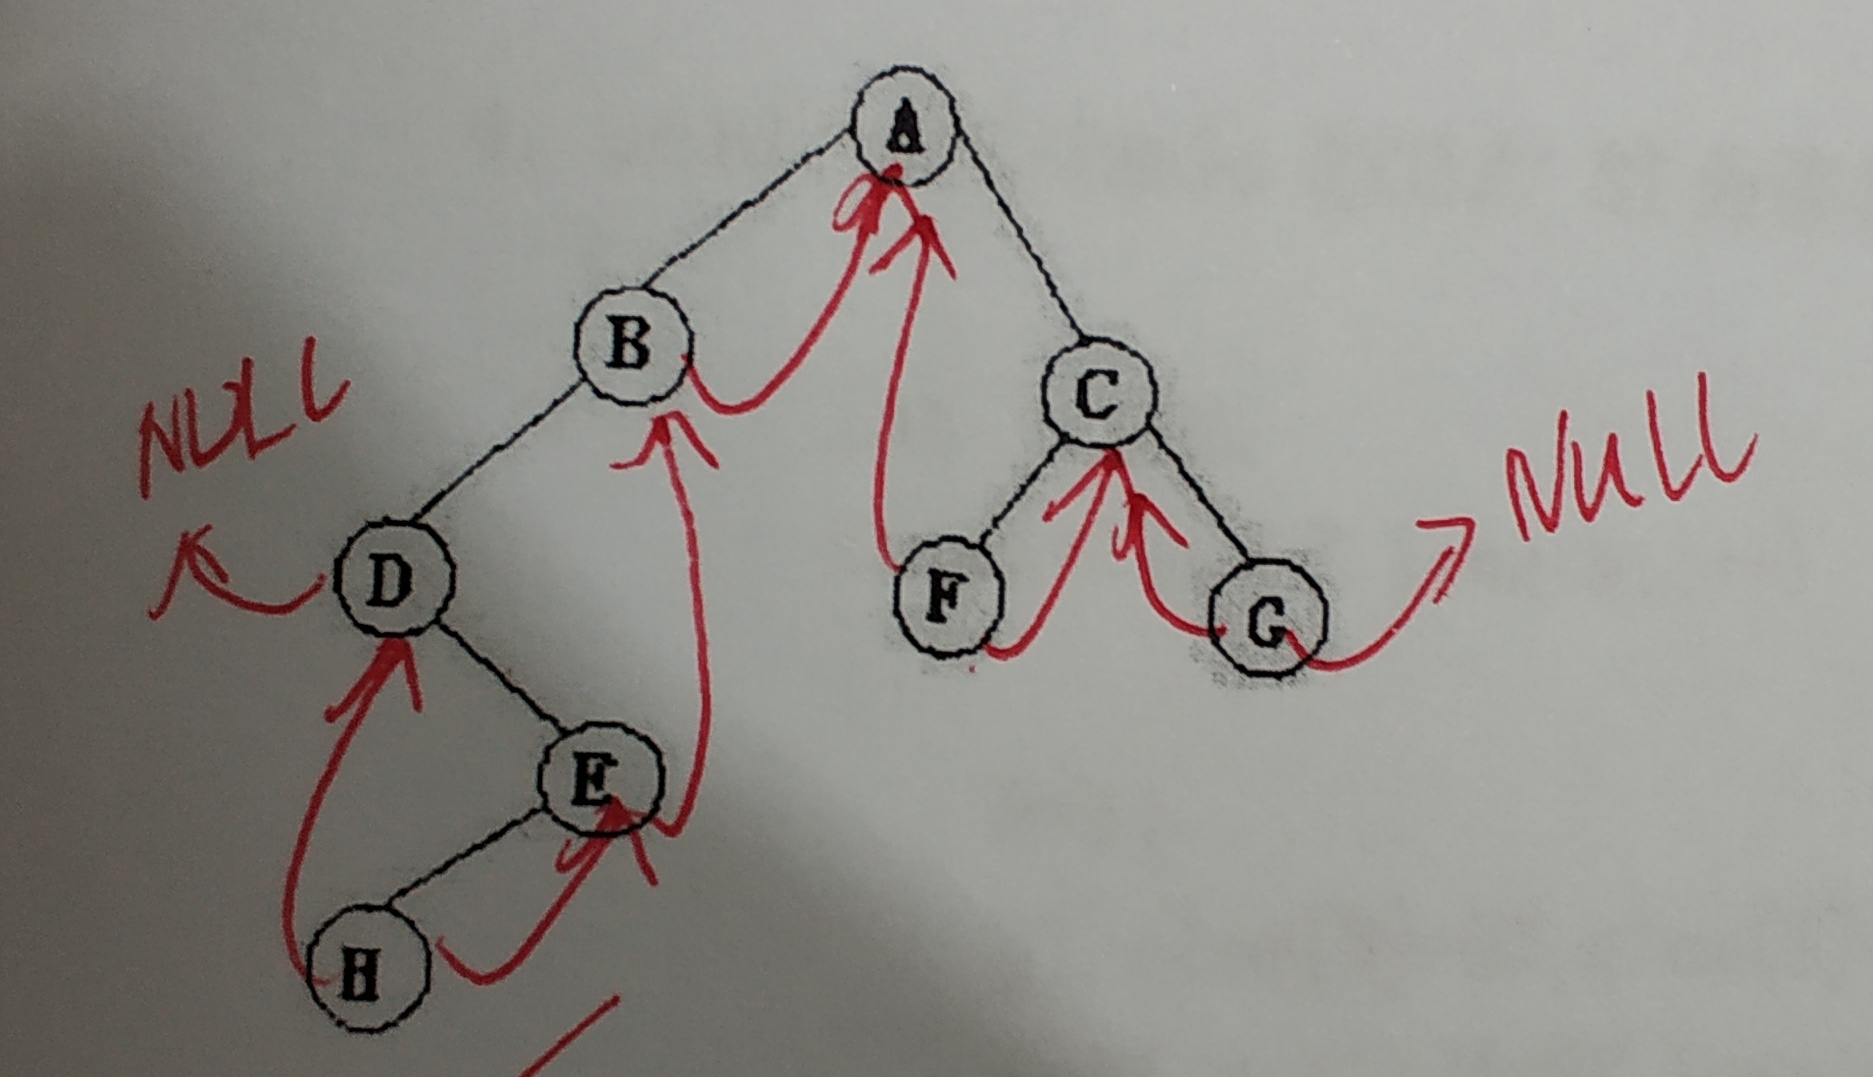
\includegraphics[scale=0.3]{example/chapter2/bitree20143ans.png}
\end{figure}


\subsection{2014年第一题}

\begin{lstlisting}[basicstyle=\small\ttfamily, caption={}, numbers=none]
已知某森林的先序遍历次序为:A,D,E,F,G,H,B,I,C,J,K,L,M,N,
中序遍历次序为:D,F,G,H,E,A,I,B,J,L,M,N,K,C
1) 画出该森林
2) 画出该森林用孩子兄弟法表示的存储结构
\end{lstlisting}
~\\
1)
~\\
详细解析\newline
DLR: {\color{red}A}{\color{blue}DEFGH}BICJKLMN\newline
LDR: {\color{blue}DFGHE}{\color{red}A}IBJLMNKC\newline
先看DLR中A表示的root节点,左边和右边分为左子树和右子树\newline
细化如果只剩下这两个\newline
DLR: {\color{blue}D}EFGH\newline
LDR: {\color{blue}D}FGHE\newline
说明D是root节点且没有左子树\newline
DLR:{\color{blue}E}FGH\newline
LDR:FGH{\color{blue}E}\newline
说明 E 是root节点且没有右子树\newline
DLR:F G H\newline
LDR:F G H\newline
他们顺序相同表示的是只有右子树的序列\newline
以此类推\newline
\begin{figure}[H]
	\centering  % 环境中的内容居中排版
	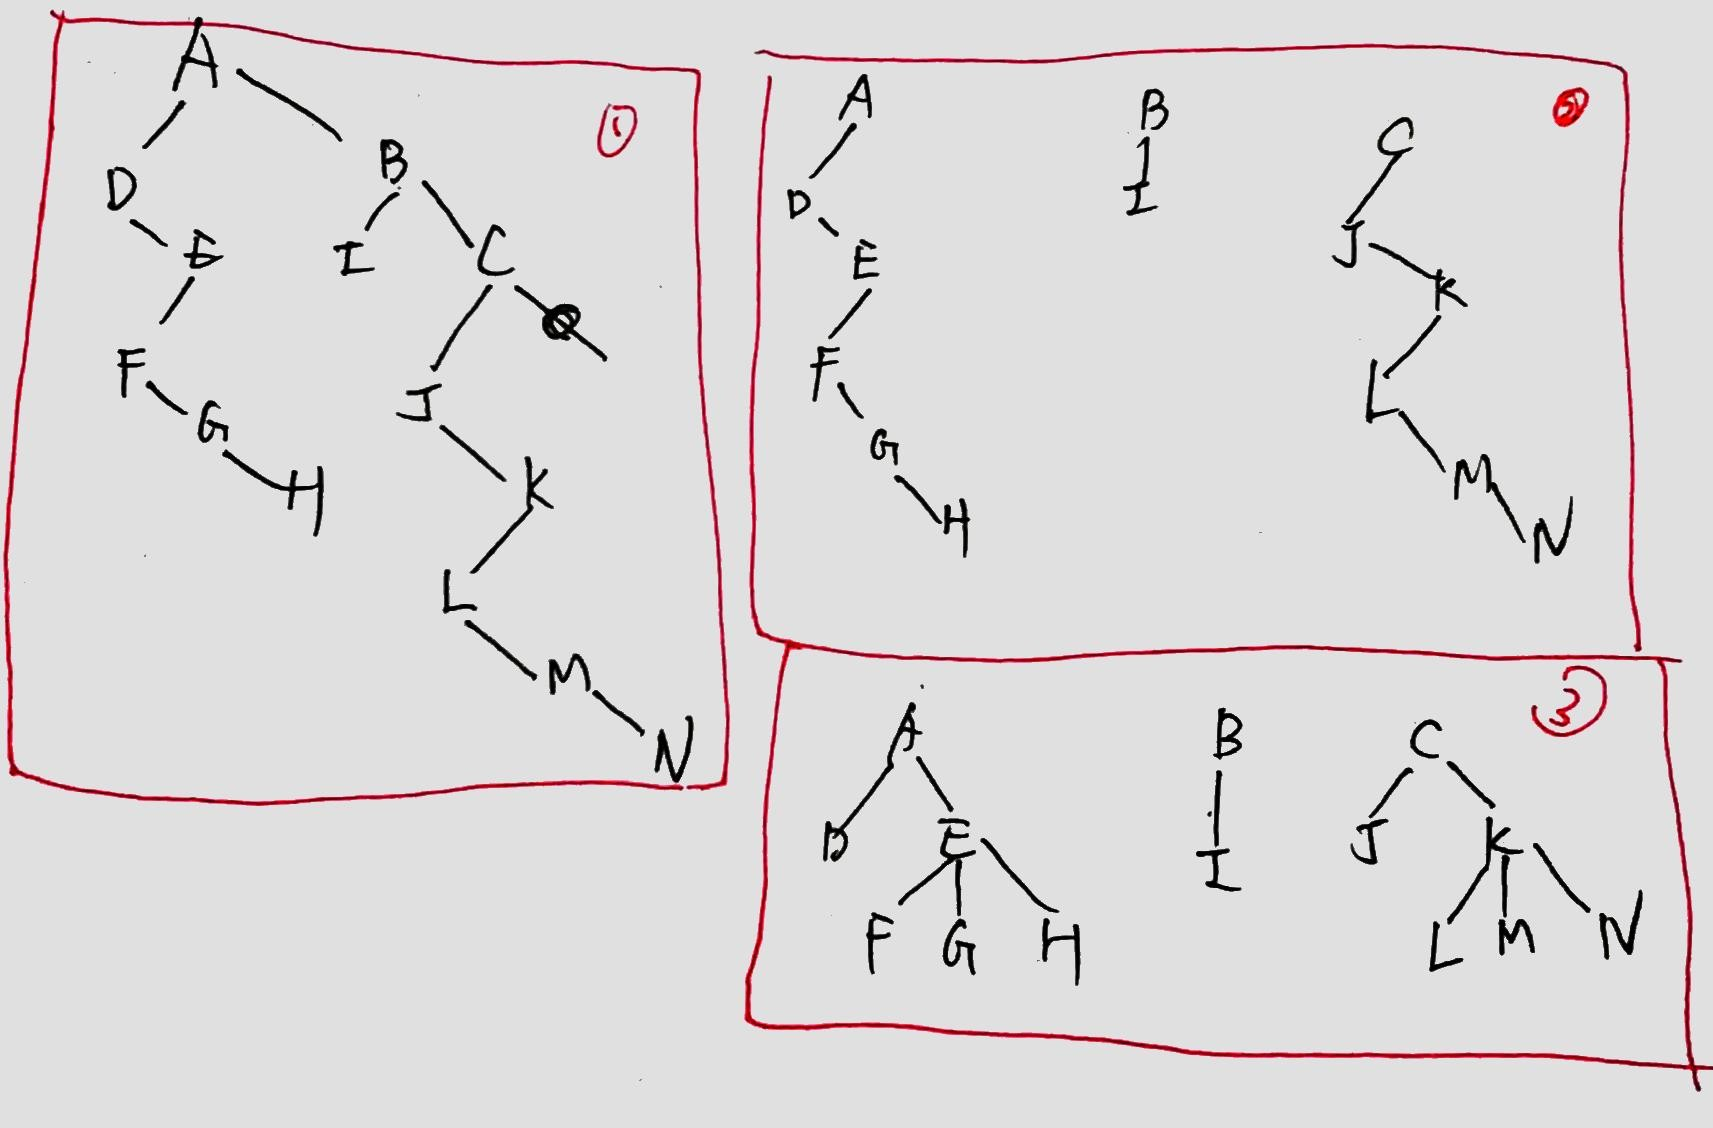
\includegraphics[scale=0.3]{example/chapter2/Img_181127155705826-1.jpg}
\end{figure}
~\\
2)
~\\
因为是孩子兄弟表示法所以存储结构是

\begin{figure}[H]
	\centering  % 环境中的内容居中排版
	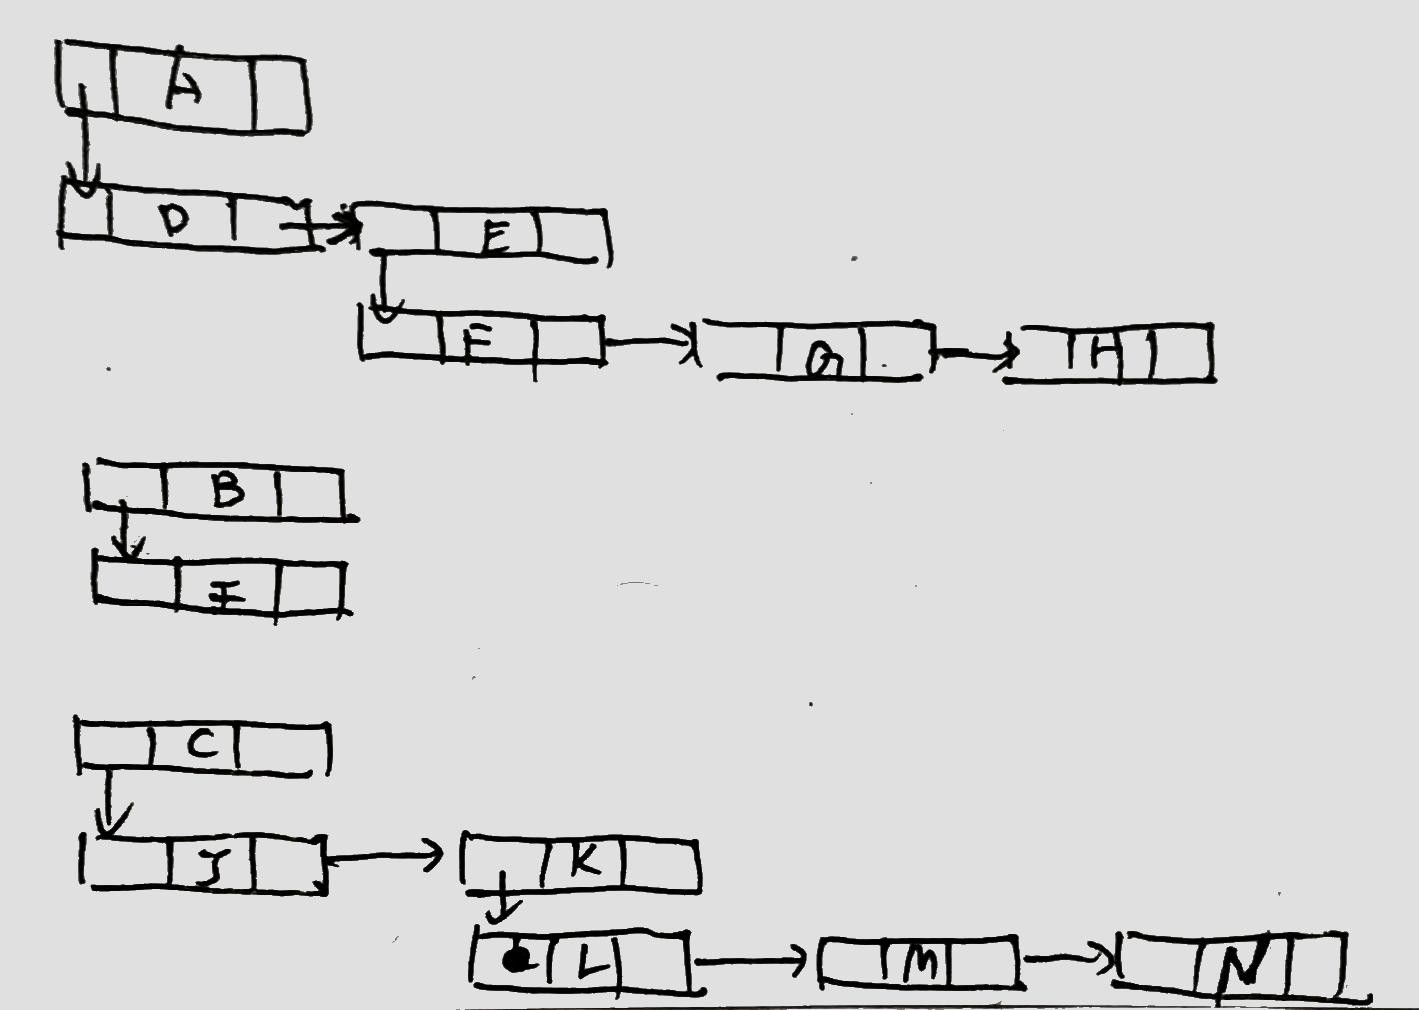
\includegraphics[scale=0.3]{example/chapter2/Img_181127161017119-1.jpg}
\end{figure}

\subsection{2015(1)}

\begin{figure}[H]
	\centering  % 环境中的内容居中排版
	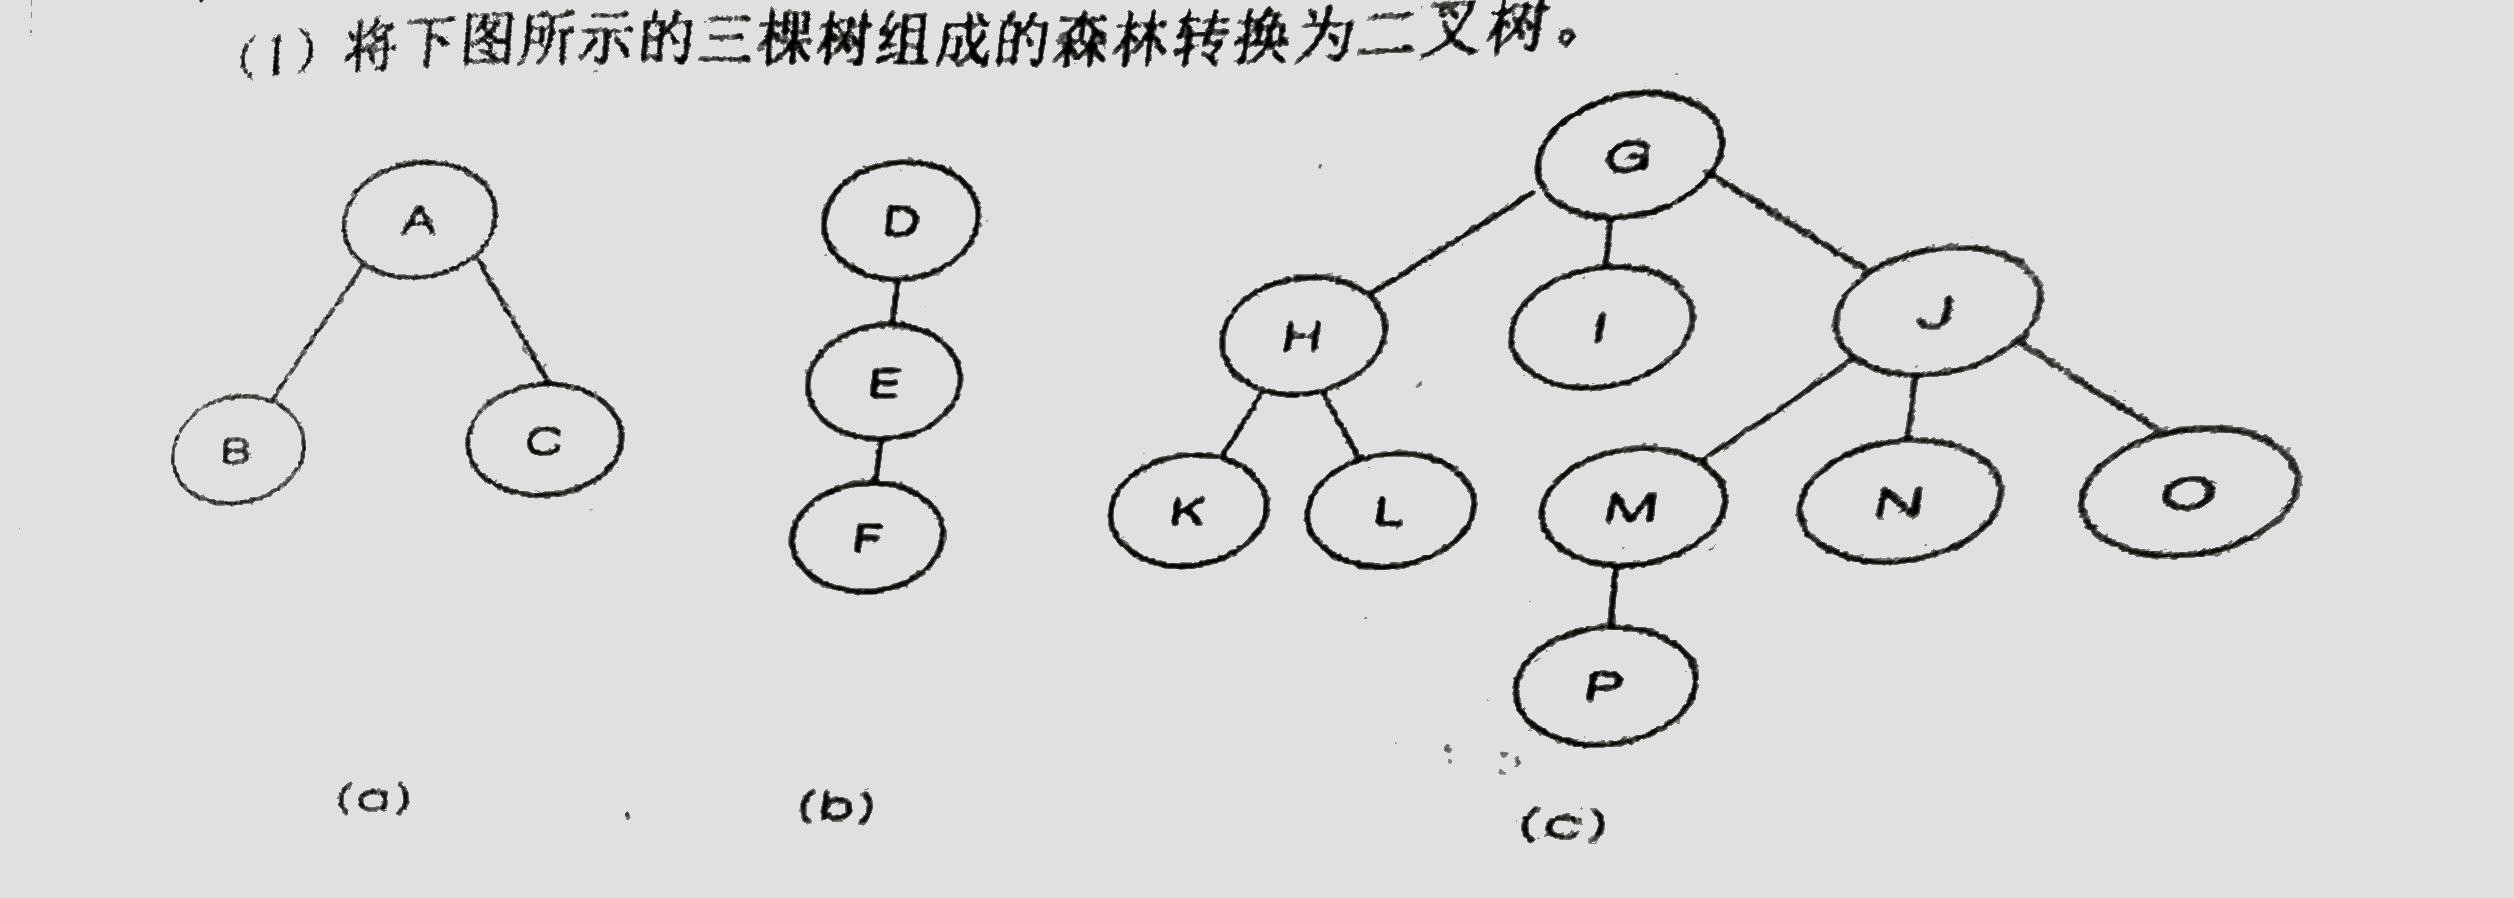
\includegraphics[scale=0.3]{example/chapter2/Img_181127161553384-1.jpg}
\end{figure}

解:

\begin{figure}[H]
	\centering  % 环境中的内容居中排版
	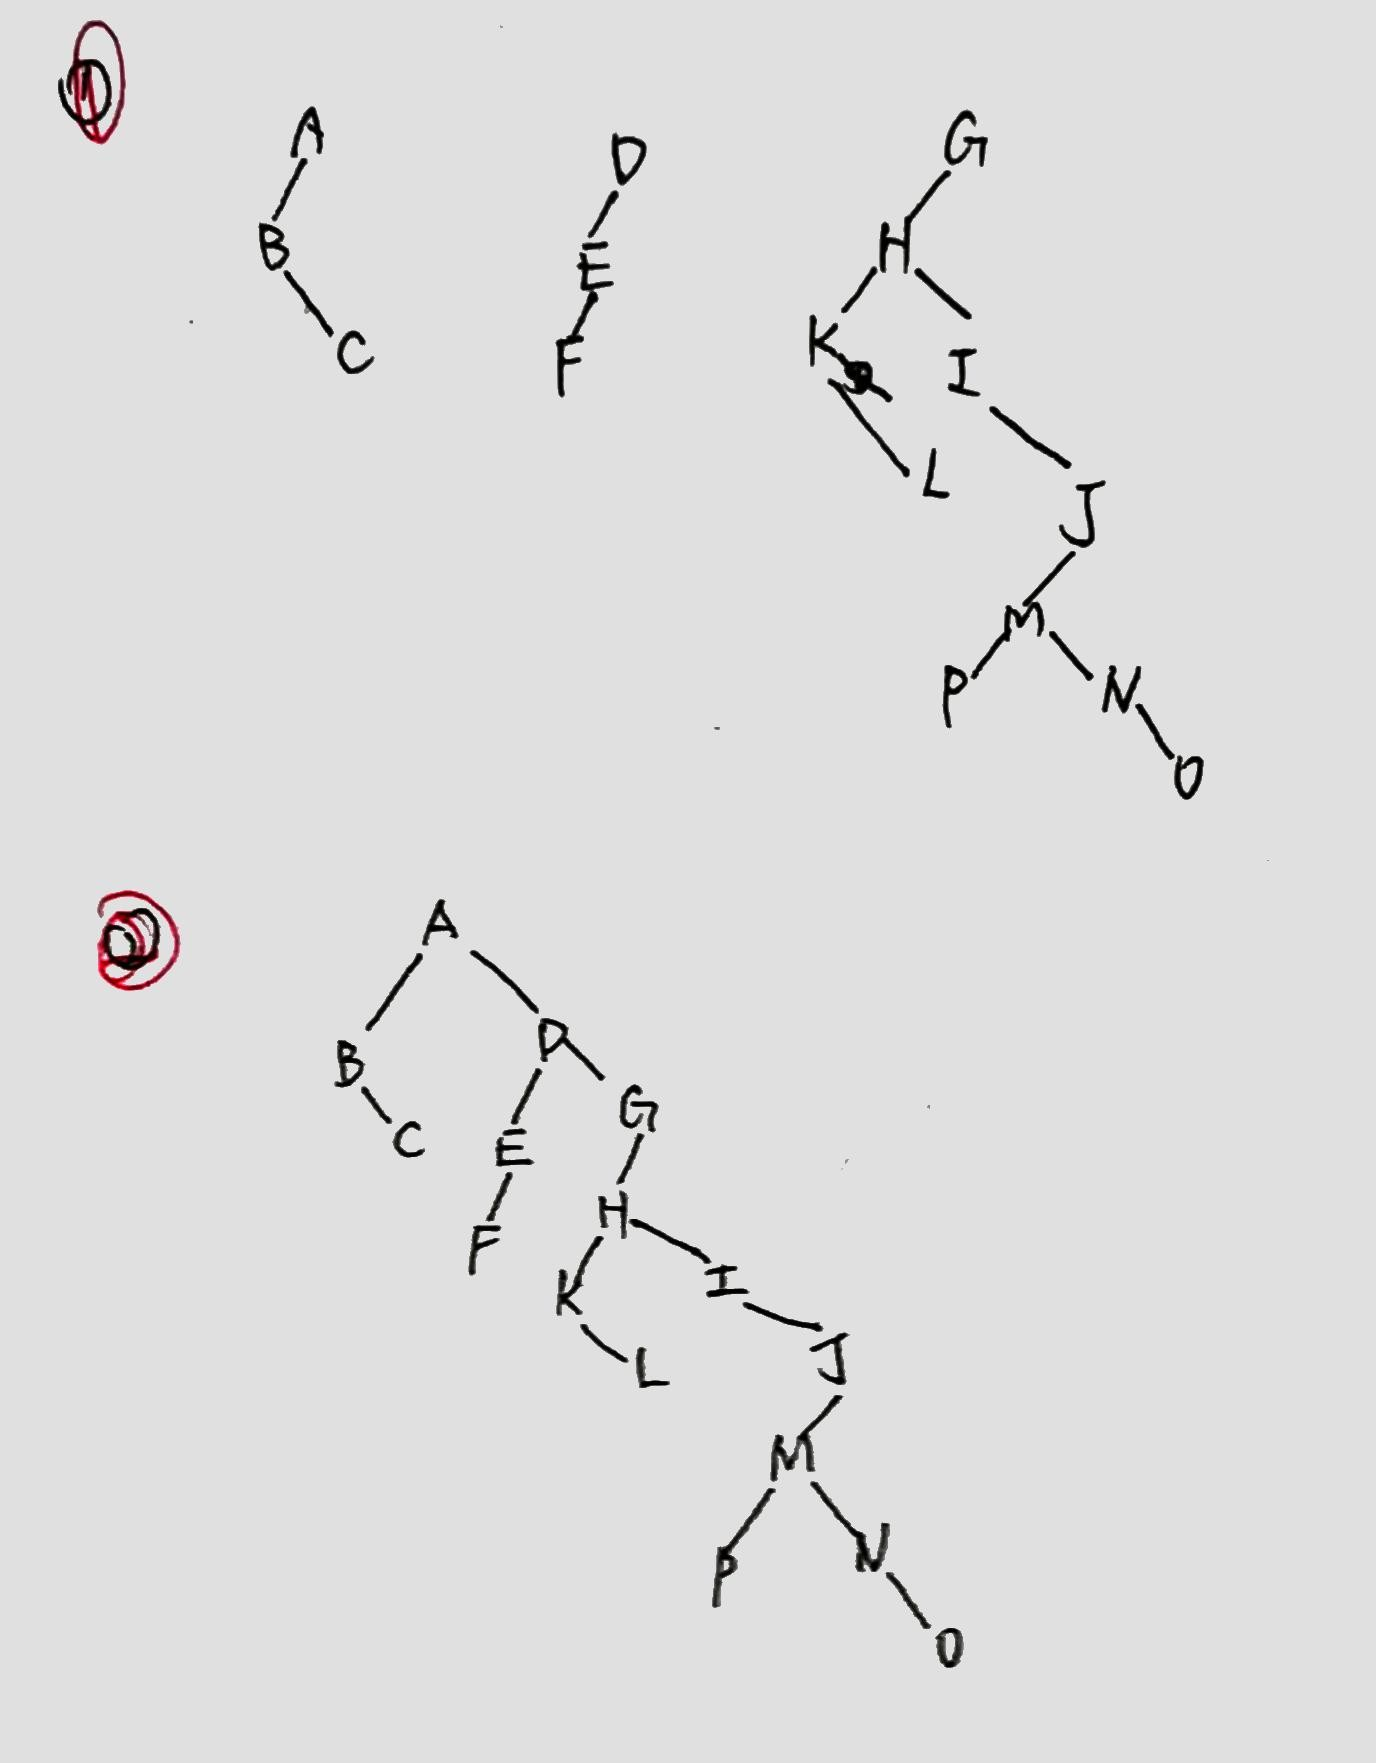
\includegraphics[scale=0.3]{example/chapter2/Img_181127161929409-1.jpg}
\end{figure}


\subsection{2016(2)}

\begin{figure}[H]
	\centering  % 环境中的内容居中排版
	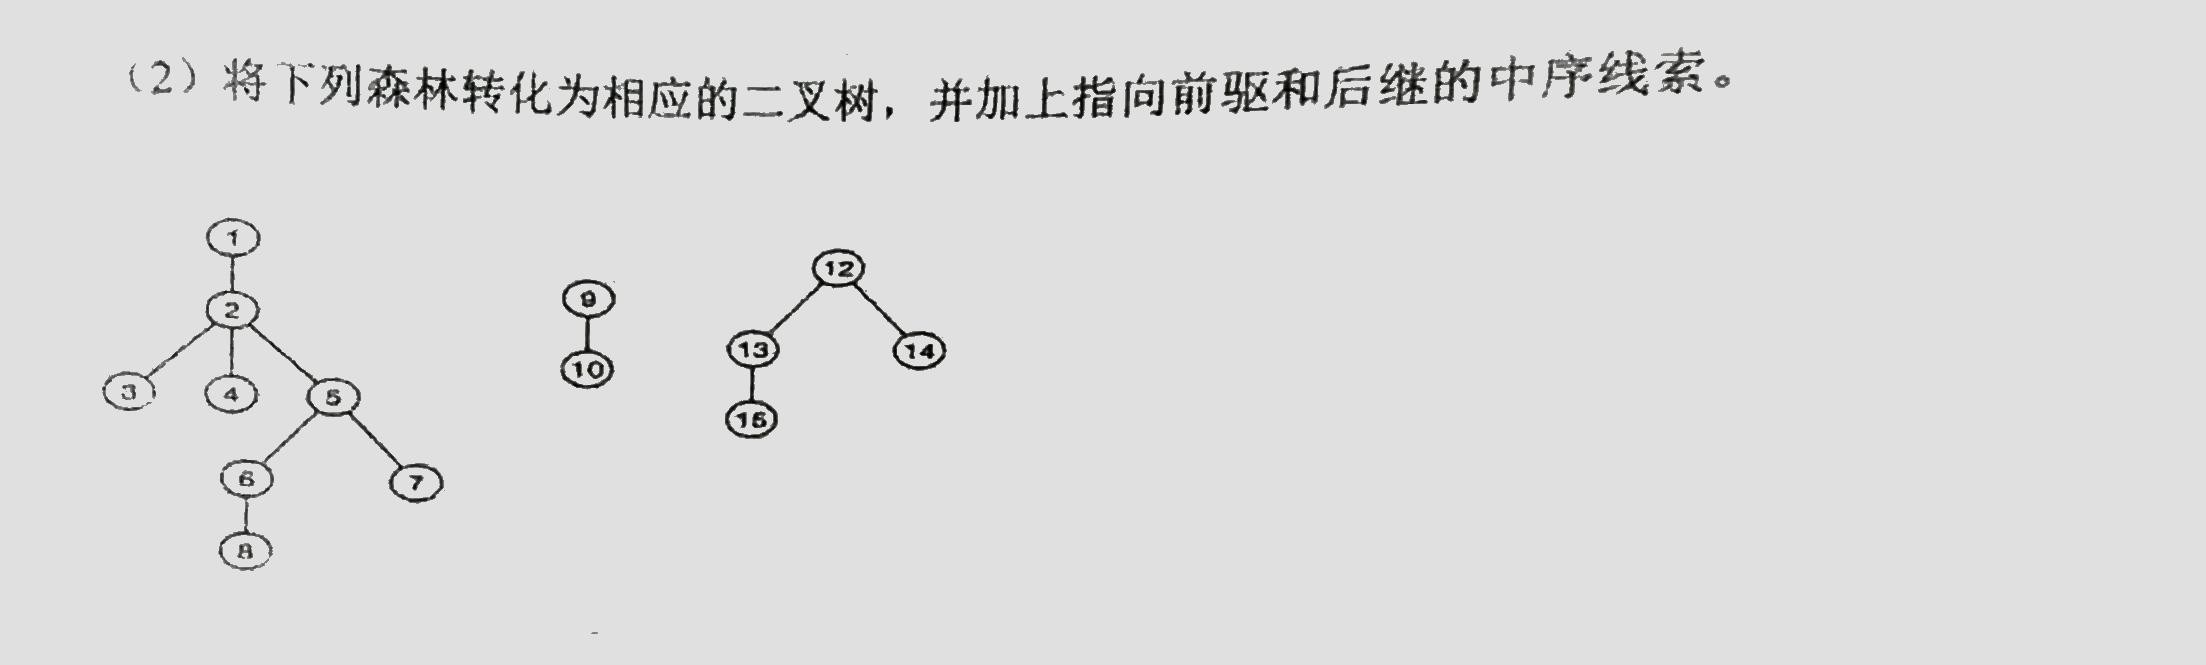
\includegraphics[scale=0.3]{example/chapter2/Img_181127162304566-1.jpg}
\end{figure}

解:

\begin{figure}[H]
	\centering  % 环境中的内容居中排版
	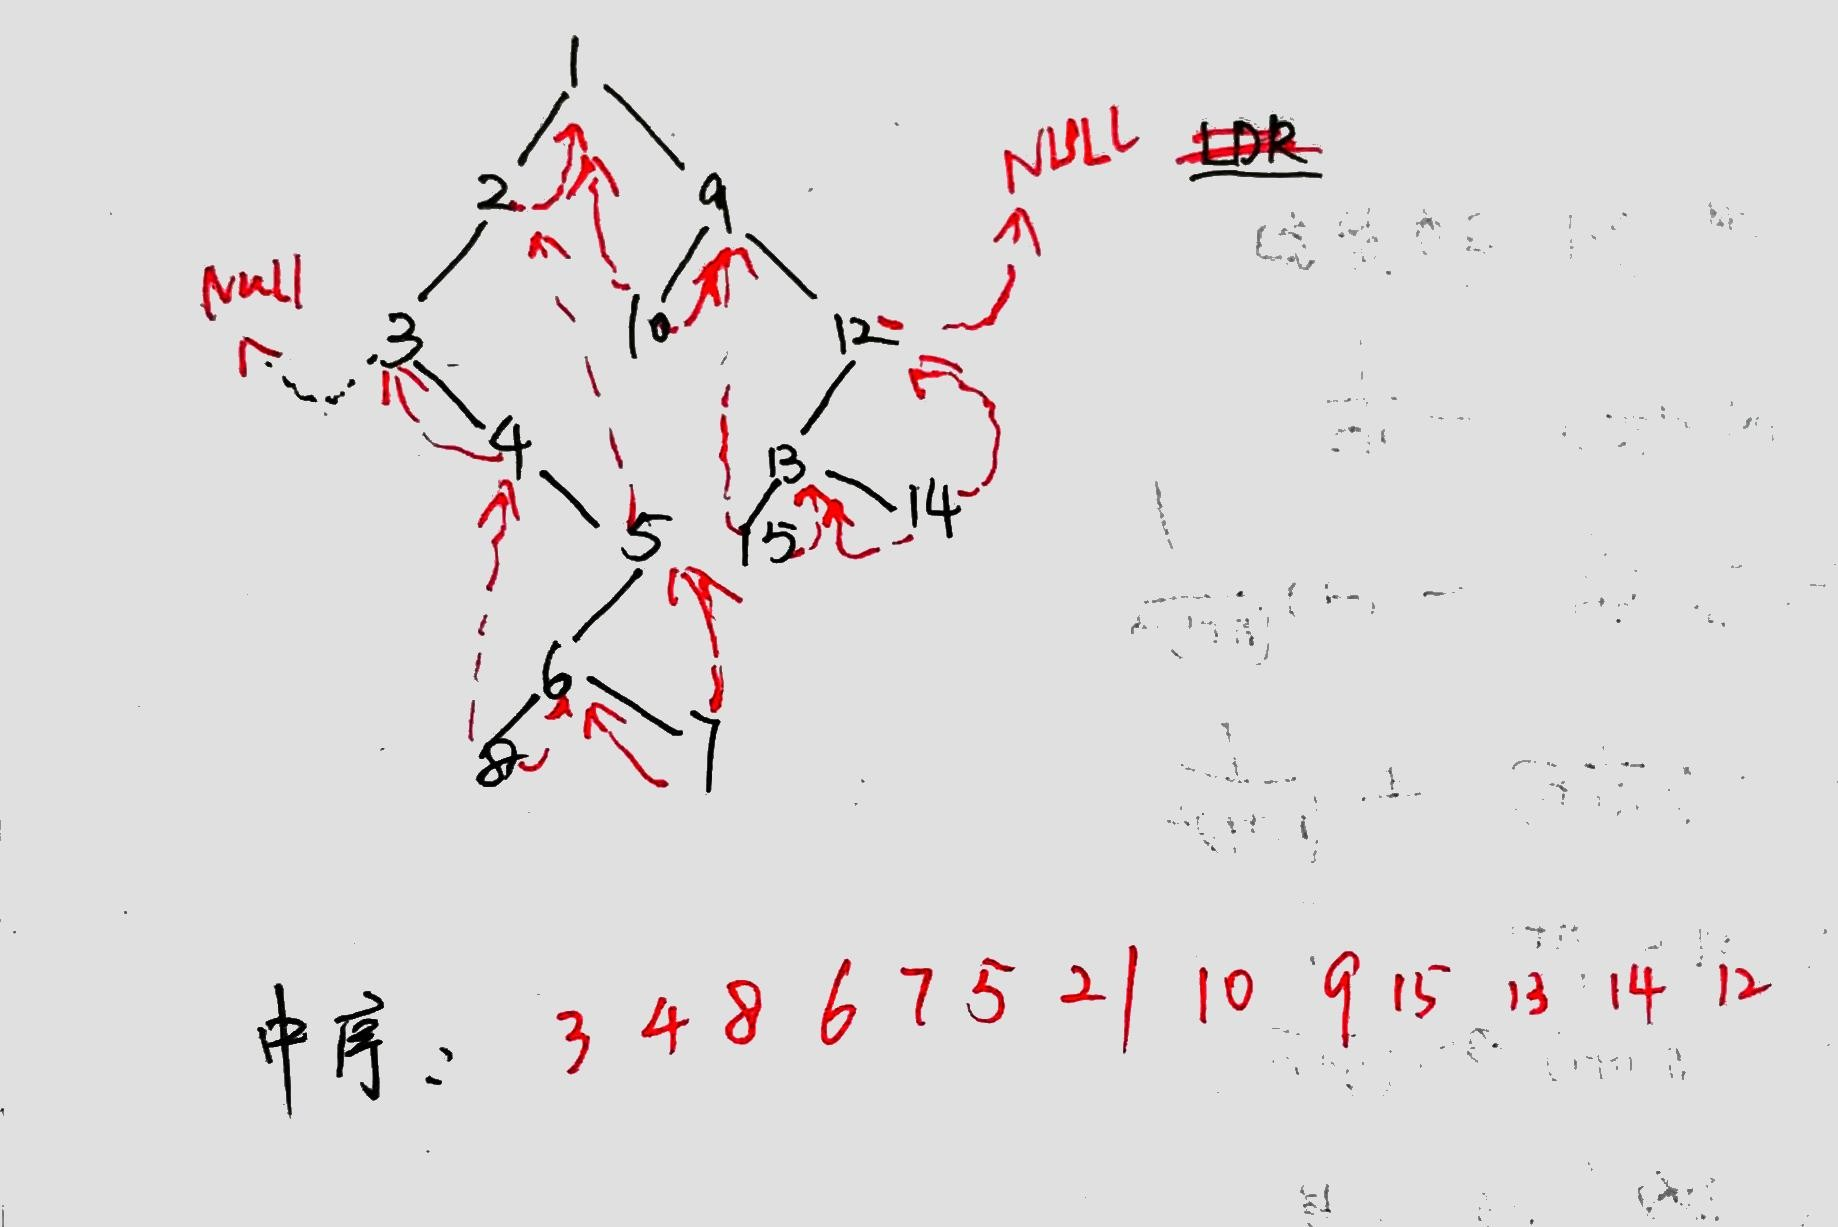
\includegraphics[scale=0.3]{example/chapter2/Img_181127163657518-1.jpg}
\end{figure}

\subsection{2017(2)}

\begin{figure}[H]
	\centering  % 环境中的内容居中排版
	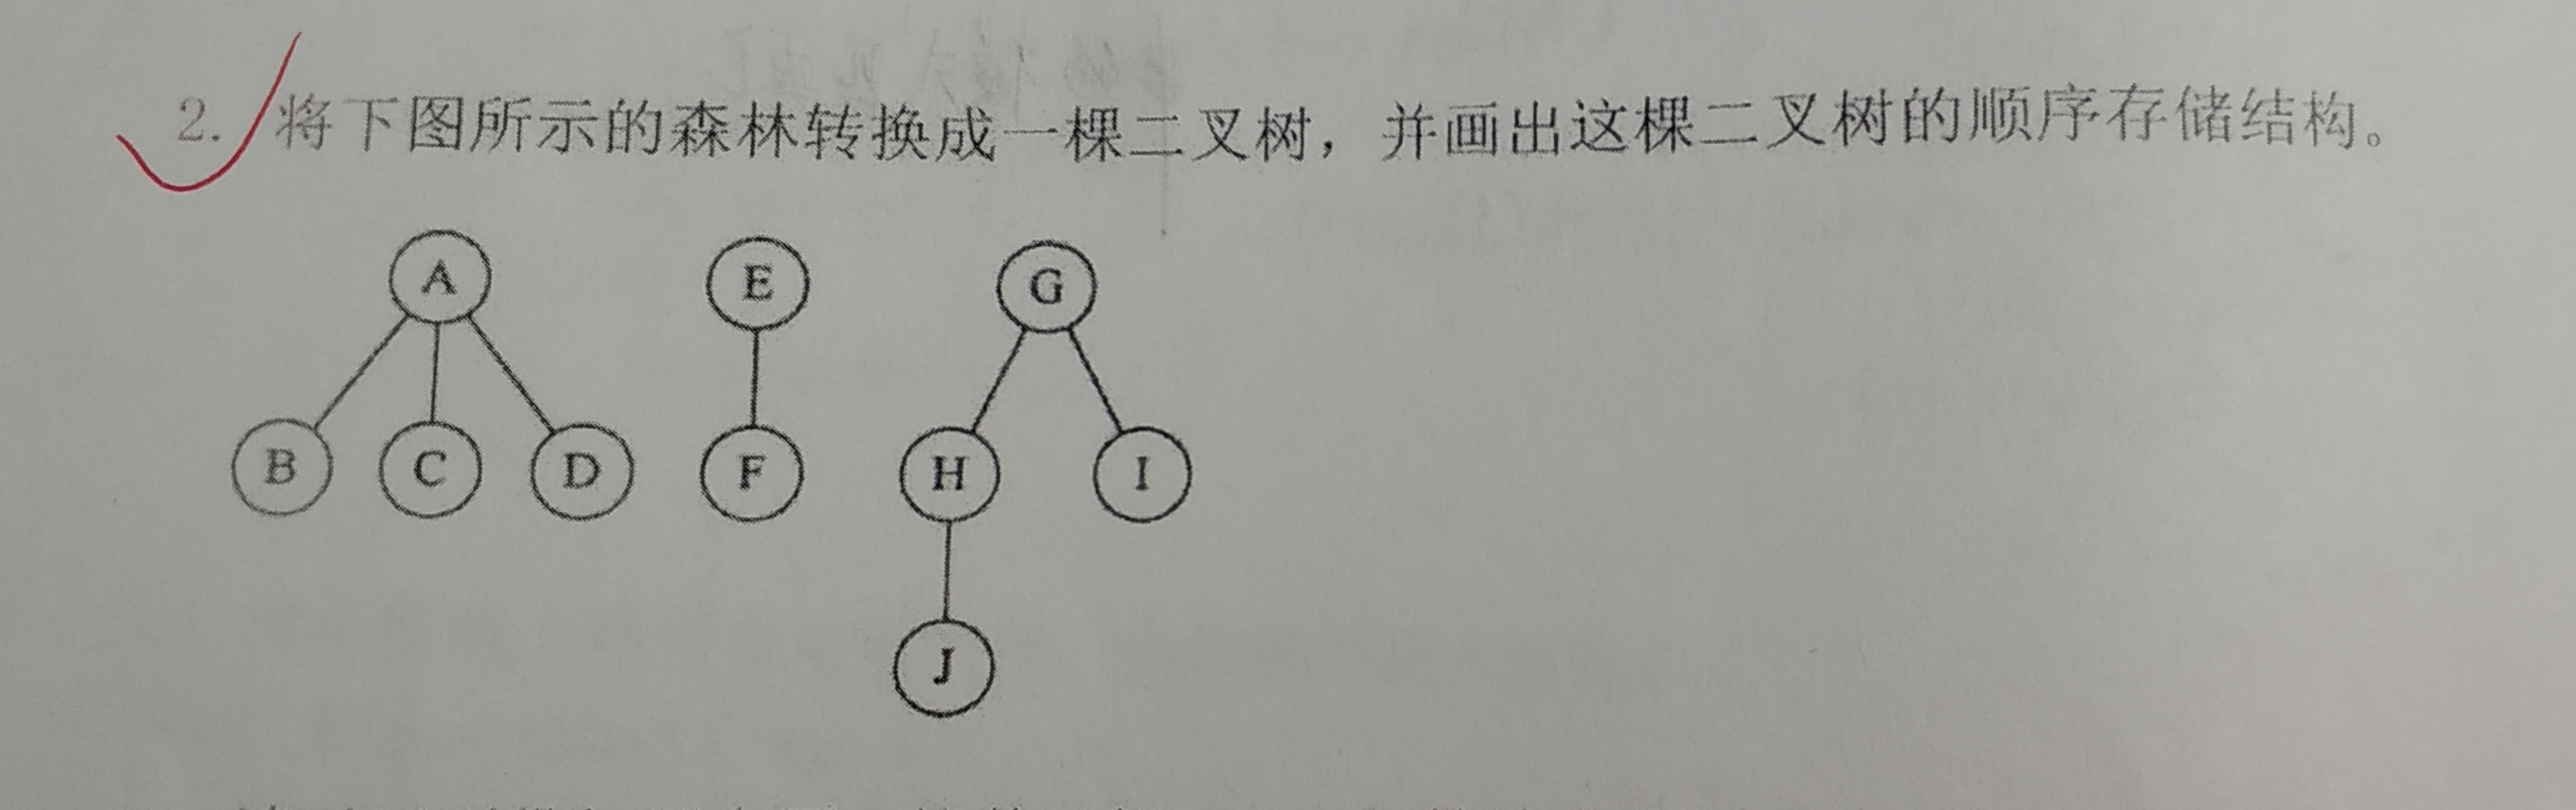
\includegraphics[scale=0.1]{example/chapter2/IMG_20181127_164746.png}
\end{figure}

解:


\begin{figure}[H]
	\centering  % 环境中的内容居中排版
	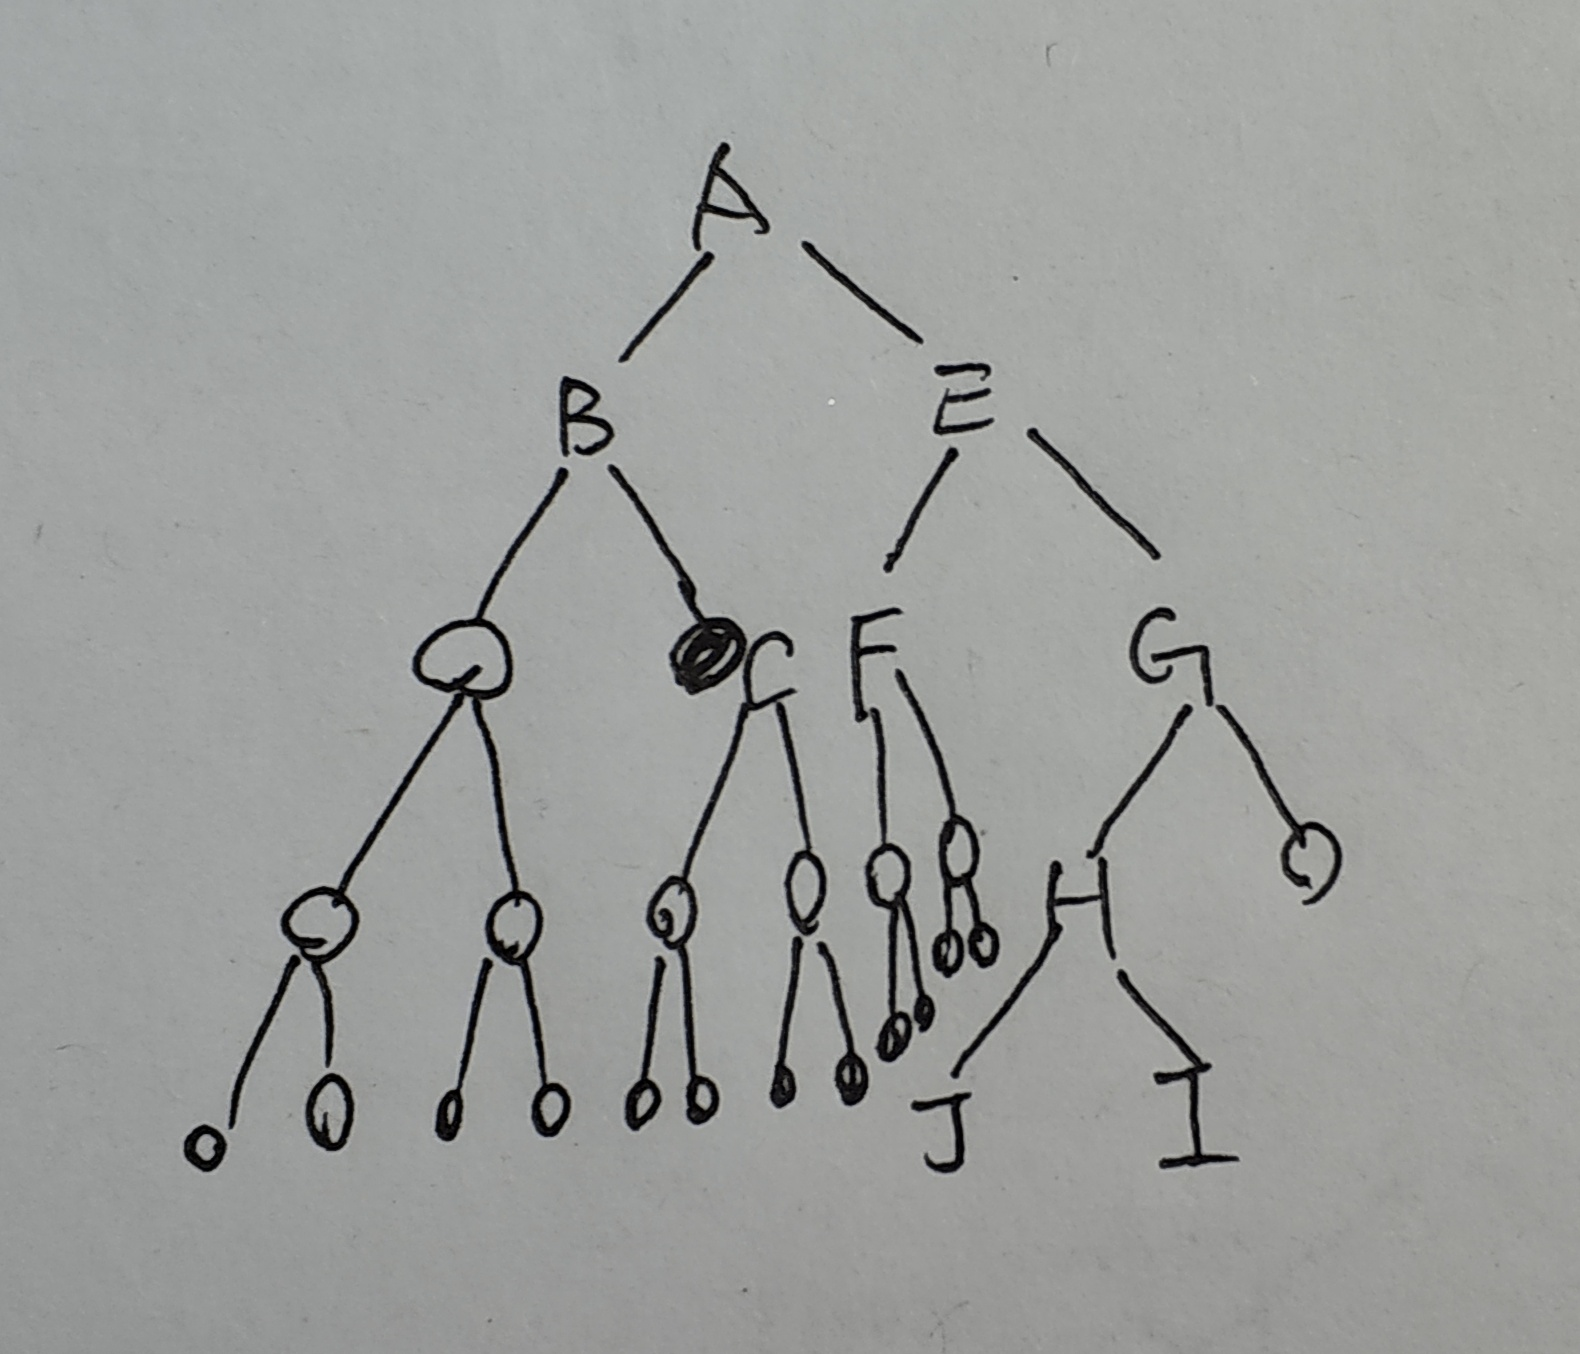
\includegraphics[scale=0.3]{example/chapter2/IMG_20181127_170103.png}
\end{figure}
~\\
顺序存储结构如下\newline
\begin{center}
\begin{tabular}{|c|c|c|c|c|c|c|c|c|c|}% 通过添加 | 来表示是否需要绘制竖线
	\hline  % 在表格最上方绘制横线
	0 & 1 & 2 & 3 & 4 & 5 & 6 & 7 & 8 & 9 \\
	\hline  % 在表格最上方绘制横线
	A & B & E &   & C & F & G &   &   &   \\
	\hline  % 在表格最上方绘制横线
	10 & 11 & 12 & 13 & 14 & 15 & 16 & 17 & 18 & 19 \\
	\hline  %在第一行和第二行之间绘制横线
	  &   &   & H &   &   &   &   &   &   \\
	\hline  % 在表格最上方绘制横线
	20 & 21 & 22 & 23 & 24 & 25 & 26 & 27 & 28 & 29 \\
	\hline  % 在表格最上方绘制横线
	  &   &   &   &   &   &   &  j & i  &   \\
	\hline  %在第一行和第二行之间绘制横线
\end{tabular}
\end{center}


\subsection{2011408}
若一棵完全二叉树有768个节点,则该二叉树中叶节点的个数是(   )\newline
解:\newline
1 + 2 + 4 + 8 + 16 + 32 + 64 + 128 +256 + 512 > 768\newline
1 + 2 + 4 + 8 + 16 + 32 + 64 + 128 +256 < 768\newline
$\frac{1*(1-2^9)}{1-2} = 511$,768 - 511 = 257 , 257 / 2 = 128.5 = 129, 256 - 129 = 127, 127 + 257 = 384.\newline
\\~ 
逻辑推理太复杂,简便的方法。应用完全二叉树的公式.  $ 当 i \le \lfloor n/2 \rfloor $ 则节点i为分支节点,否则为叶子节点。\newline
得到 768 / 2 = 384, 得到  768 - 384 = 384 则有384个叶子节点。\newline


\subsection{2014年408}
二叉树的带权路径长度(WPL)是二叉树中所有叶节点的带权路径长度之和。给定一棵二叉树T,采用二叉链表存储,节点结构为:'[left, weight, right]'其中叶节点的weight域保存该节点的非负权值、设root为指向T的根节点的指针,请设计求T的WPL的算法,要求:\newline
1) 给出算法的基本设计思想;\newline
2) 使用C或C++语言,给出二叉树节点的数据类型定义;\newline
3) 根据设计思想,采用C或C++语言描述算法,关键之处给出注释.\newline
解:\newline
1)\newline
设计思想是:层次遍历一层如果遇到是叶节点,那么计算这个节点的带权路径长度。\newline
\begin{lstlisting}[basicstyle=\small\ttfamily, caption={}, numbers=none]
#include <iostream>
#include <queue>
using namespace std;
typedef struct LNode {
	LNode *left;
	LNode *right;
	int weight;
}LNode;

int calcWPL(LNode *root) {
	queue<LNode*> q;
	q.push(root);
	q.push(NULL);
	int level = 1;
	int wpl = 0;
	while (!q.empty()) {
		LNode * out = q.front();
		//cout << out->weight << endl;
		//确定是第几层,加入特殊的符号
		if (out == NULL) {
			level++;
			q.pop();
			if (q.empty()) {
				break;
			}
			out = q.front();//新的层的新的元素
			q.pop();
			q.push(NULL);
		}
		else {
			q.pop();
		}
		wpl += out->weight * level;
		cout << "[DEBUG weight] " << out->weight << endl;
		if (out->left!=NULL) {
			cout << "[DEBUG left]" << out->left->weight << endl;
			q.push(out->left);
		}
		if (out->right != NULL) {
			q.push(out->right);
			cout << "[DEBUG right]" << out->right->weight << endl;
		}
	}
	return wpl;
}


int main() {
// 构建二叉树
	LNode * root = (LNode *)malloc(sizeof(LNode));
	LNode * left1 = (LNode *)malloc(sizeof(LNode));
	LNode * right1 = (LNode *)malloc(sizeof(LNode));
	LNode * left1right = (LNode *)malloc(sizeof(LNode));
	LNode * left1left = (LNode *)malloc(sizeof(LNode));
	root->weight = 1; root->left = left1; root->right = right1;
	left1->weight = 2; left1->left = left1left; left1->right = left1right;
	right1->weight = 3; right1->left = NULL; right1->right = NULL;
	left1right->weight = 5; left1right->left = NULL; left1right->right = NULL;
	left1left->weight = 4; left1left->left = NULL; left1left->right = NULL;
	//
	cout << "WPL is: " << calcWPL(root) << endl;
	system("pause");
}
\end{lstlisting}
参考链接层次遍历寻找特定的层:\url{https://blog.csdn.net/OrthocenterChocolate/article/details/37612183}\newline
当然,先序遍历的方式更好。\newline
\begin{lstlisting}[basicstyle=\small\ttfamily, caption={}, numbers=none]
int WPL(BiTree Root){
	return wpl_PreOrder(root, 0);
}
int wpl_PreOrder(BiTree root, int deep){
	static int wpl = 0;
	if(root->lchild==NULL&&root->rchild==NULL){
		wpl+=deep*root->weight;
	}
	if(root->lchild!=NULL){
		wpl_PreOrder(root->lchild, deep+1);
	}
	if(root->rchild!=NULL){
		wpl_PreOrder(root->rchild, deep+1);
	}
	return wpl;
}
\end{lstlisting}

\subsection{2016年408选择题}
若森铃F有15条边、25个节点,则F包含树的个数是(  ) \newline
解:\newline
25 - 15 = 10 ==> 有10棵树。

\subsection{2011年408 \&\&  杭电2019年选择题}
已知一棵有2011个节点的树,其叶节点个数为116,该树对应的二叉树中五右孩子的结点个数是(   )\newline
A. 115  B. 116  C. 1895  D. 1896\newline














